\documentclass[12pt,twoside]{report}
\usepackage[a4paper,width=150mm,top=25mm,bottom=25mm,bindingoffset=6mm]{geometry}
\usepackage[english]{babel}

\setlength{\headheight}{15pt} 

\usepackage[utf8]{inputenc}
%\usepackage[latin1]{inputenc}
\usepackage{fancyhdr}
\usepackage{indentfirst}
\usepackage{graphicx}
\graphicspath{ {Images/}  }
\usepackage{newlfont}
\usepackage{amssymb}
\usepackage{amsmath}
\usepackage{latexsym}
\usepackage{amsthm}
\usepackage{listings}
\usepackage{xcolor}
\usepackage{mdframed}
\usepackage{epigraph}
\usepackage{csquotes}

\usepackage{hyperref}

\usepackage{makecell}
\usepackage{tabularx}
%\usepackage{booktabs}
% \usepackage{graphicx}

\usepackage{tabulary}
\usepackage{epsf} 

\usepackage{breqn}

\usepackage[backend=biber]{biblatex}
\addbibresource{references.bib}

\usepackage{array}
\usepackage{tabu}

\usepackage{amsmath}
\usepackage{amssymb}


\usepackage{lipsum}

%\usepackage{pgf-pie}


%\usepackage{pgfplots}

%\pgfplotsset{
 % compat=newest,
  %xlabel near ticks,
 % ylabel near ticks
%}

\pagestyle{fancy}\addtolength{\headwidth}{20pt}
\renewcommand{\chaptermark}[1]{\markboth{\thechapter.\ #1}{}}
\renewcommand{\sectionmark}[1]{\markright{\thesection \ #1}{}}
\rhead[\fancyplain{}{\bfseries\leftmark}]{\fancyplain{}{\bfseries\thepage}}
\cfoot{}
\linespread{1.3}  
\begin{document}

\begin{titlepage}               

\thispagestyle{empty}                  
\topmargin=6.5cm                        
\raggedleft                            	
\large                                 		
\em                                    
%Questa \`e la \textsc{Dedica}:\\
%ognuno pu\`o scrivere quello che vuole, \\
%anche nulla \ldots     
%INTA 'NA SAMANA NASCE 'NU ZITEDU E DICE: CIAO PAPA!
-
\newpage                            
\clearpage{\pagestyle{empty}\cleardoublepage}
\end{titlepage}
\pagenumbering{roman}                   
\chapter*{Abstract}             
\rhead[\fancyplain{}{\bfseries
Abstract}]{\fancyplain{}{\bfseries\thepage}}
\lhead[\fancyplain{}{\bfseries\thepage}]{\fancyplain{}{\bfseries
Abstract}}

%%%%%%%%%%%%%%%%%%%%%%%%%%%%%%%%%%%%%%%%%aggiunge la voce Introduzione
                                        %   nell'indice
\addcontentsline{toc}{chapter}{Abstract}
%\input{Introduction}
%%%%%%%%%%%%%%%%%%%%%%%%%%%%%%%%%%%%%%%%%non numera l'ultima pagina sinistra
\clearpage{\pagestyle{empty}\cleardoublepage}

%\rhead[\fancyplain{}{\bfseries\thepage}]{\fancyplain{}{\bfseries
%INDICE}}
\rhead[\fancyplain{}{\bfseries\leftmark}]{\fancyplain{}{\bfseries\thepage}}
\lhead[\fancyplain{}{\bfseries\thepage}]{\fancyplain{}{\bfseries
INDICE}}
\tableofcontents                        %crea l'indice
%%%%%%%%%%%%%%%%%%%%%%%%%%%%%%%%%%%%%%%%%imposta l'intestazione di pagina


%%%%%%%%%%%%%%%%%%%%%%%%%%%%%%%%%%%%%%%%%non numera l'ultima pagina sinistra
\clearpage{\pagestyle{empty}\cleardoublepage}
\listoffigures                          %crea l'elenco delle figure
%%%%%%%%%%%%%%%%%%%%%%%%%%%%%%%%%%%%%%%%%non numera l'ultima pagina sinistra
\clearpage{\pagestyle{empty}\cleardoublepage}
\listoftables                           %crea l'elenco delle tabelle
%%%%%%%%%%%%%%%%%%%%%%%%%%%%%%%%%%%%%%%%%non numera l'ultima pagina sinistra
\clearpage{\pagestyle{empty}\cleardoublepage}
%%%%%%%%%%%%%%%%%%%%%%%%%%%%%%%%%%%%%%%%%imposta l'intestazione di pagina


\lhead[\fancyplain{}{\bfseries\thepage}]{\fancyplain{}{\bfseries\rightmark}}

\pagenumbering{arabic}                  %mette i numeri arabi


\chapter{Background}

In this chapter we are going to present the existing Cowbird framework realized within the SWAN project \cite{swanonline}. Cowbird is a flexible and energy efficient framework for building Android application that use both smartphone sensors and IoT sensors\cite{cowbirdarticle}. Cowbird extends the SWAN framework \cite{swanphd} and it supports context-based expressions (queries) that can run both on a smartphone and in the cloud; with the Cowbird framework, developers can easily decide where to perform the computation according to the source of the data and the frequency of the updates.

\section{The SWAN framework}
SWAN (Sensing With Android Nodes) is a framework for easily building context-aware applications for Android smartphones \cite{swanphd}. The framework provides application developers a high-level abstraction for accessing smartphone's sensors. In particular, the SWAN framework is designed to be executed as an Android background service and it acts as a middleware between applications and sensors: running applications can access it through a well-defined API. The SWAN framework reduces storage redundancy and code duplication caused by multiple sensor-based applications running simultaneously. In fact, it provides a centralized solution for collecting and storing data from sensors. 

\subsection{SWAN sensors}
One of the most important characteristic of SWAN is its \emph{multi sensor support}; in fact, at the moment, SWAN supports more than 20 different types of sensors. We can distinguish two different categories of sensors:
\begin{itemize}
\item	 \emph{Hardware sensors}. The physical sensors installed on the devices (e.g. accelerometer, GPS, etc.).
\item \emph{Software sensors}. Software \emph{data sources} (e.g. calendar, rain prediction, Twitter, etc.) that can be installed on the devices or that can run somewhere else. 
\end{itemize}

SWAN sensors are implemented as background services that are responsible for gathering the sensor's data. In case of external software sensors such as the rain prediction or Twitter, the SWAN sensor continuously polls from the web endpoint to get live data. The data accuracy can be improved increasing the polling frequency. 

From an architectural point of view all the SWAN sensors run in separate processes in order to remain unaffected if the application built on top of SWAN crashes: this design approach prevents data losses. The communication between SWAN sensors and the other components is performed through inter-process communication (IPC).

\subsection{SWAN-Song}
One of the SWAN framework core functionalities is the SWAN-Song support. SWAN-Song \cite{swansong} is a a domain specific language
for context expressions. SWAN-Song is used by applications to register expressions into SWAN. After registering an expression, SWAN evaluates it and sends back the result to the application. 

The SWAN-Song language is a form of zeroth-order logic, which allows the description of a particular combination of contextual information using sensor based expression predicates. Predicates can be combined using math, comparison, and logic operators, and a specification of a \emph{history window} and \emph{history reduction} operator.  

\subsubsection{SWAN-Song expressions \& predicates}
A SWAN-Song expression is composed of two required components and three optional components. Required are a sensor entity and a value path. Optional components are a list of one or more configuration parameters, a history window and a history reduction mode.

There are two types of SWAN expressions:
\begin{itemize}
\item \emph{Value expressions}. Such expressions return a sensor value or a list of sensor
values. As an example, the following expression gets the current light intensity:
\begin{equation} \label{eq:luxexpression}
self@light:lux\big\{MEAN, 2000ms\big\}
\end{equation}
In expression \ref{eq:luxexpression} self is the location identifier of the device, light
is the sensor name, lux is the value path, MEAN represents the history reduction mode and 2000ms indicates the history window. The expression computes the average value generated by the light sensor in the last 2000 milliseconds.

\item \emph{Tristate expressions} Such expressions are useful for defining complex context conditions and they can take one of the following values: TRUE, FALSE or UNDEFINED. An expression is evaluated to UNDEFINED if the sensor queried in the expression is turned off or not available. As an example, the following expression(s) can be used to notify the user that he/she should exercise:
\begin{equation} \label{eq:morningexpression}
Morning = self@time:hour < 12 
\end{equation}
\begin{equation} \label{eq:dryexpression}
Dry = self@rain:expected == 0 
\end{equation}
\begin{equation} \label{eq:mobilityexpression}
Mobility = self@movement:total \big\{MAX,3600000\big\} > 15.0
\end{equation}
\begin{equation} \label{eq:exerciseexpression}
Exercise = Morning \text{ \&\& } Dry \text{ \&\& }  \text{!} (Mobility)
\end{equation}
\end{itemize}
The \emph{Morning} expression \ref{eq:morningexpression} uses the time sensor to
check if it is earlier than 12:00 pm; the \emph{Dry} expression \ref{eq:dryexpression}, instead, checks the live rain prediction using the rain sensor and \emph{Mobility} \ref{eq:mobilityexpression} uses the accelerometer sensor to check if the user has been moving in the past hour. The \emph{Exercise} expression \ref{eq:exerciseexpression} combines the other TriState expressions to determine whether or not the context of the user is suitable for a workout.

Because of the time windowing of sensor values, sensor predicates represent an array of \emph{time-stamped values}. History operators are then applied on these values collected within the time specified time frame. SWAN-Song expressions support different history reduction modes, such as:
\begin{itemize}
\item ALL. This operator checks if \emph{all} the time-stamped values, sensed within the time window, match the condition defined in the SWAN-Song expression.
\item ANY. Selects any value that makes the comparison \emph{true} as the value of the sensor. The ANY operator is also the default history reduction mode.
\item MIN, MAX, MEAN, and MEDIAN, which will select or calculate the appropriate value.
\end{itemize}

\subsection{Architecture}
As already mentioned, applications can register SWAN-Song expressions using the SWAN API. On registering a new expression, a component named the Expression Evaluation Engine (see Figure \ref{fig:cowbird_architecture}) is invoked. The Expression Evaluation Engine is responsible for evaluating SWAN-Song expressions: it interacts with the sensors in order to fetch the sensed data and compute the result of the expressions. Whenever new sensed data is available, it is sent to the Expression Evaluation Engine, which processes it and sends the result back to the application.

 \begin{figure}[ht!]
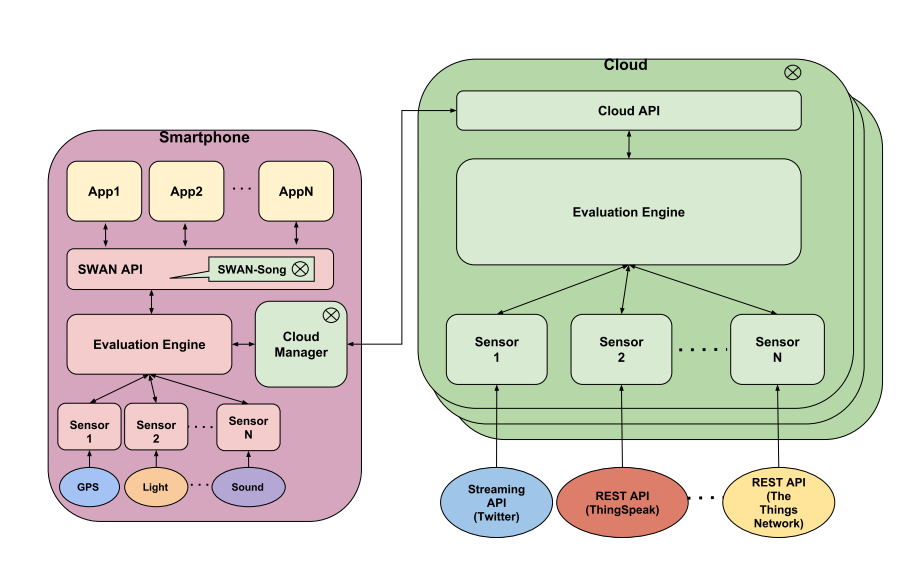
\includegraphics[width=1\textwidth]{images/cowbird_architecture.png}
 \caption{SWAN and Cowbird architecture. Cowbirds components are marked with $\otimes$. Source: \cite{cowbirdarticle}}
\label{fig:cowbird_architecture}
\end{figure}

\section{The Cowbird framework}
The Cowbird framework has been designed as a cloud extension of the SWAN framework. In particular, it enables the combination of smartphones sensors and real-time web data: these data can be originally generated by IoT sensors or, more in general, they can be any data which can be retrieved by polling a web resource (e.g. Twitter feeds) \cite{cowbirdarticle}. Furthermore, the Cowbird framework reduces the overall communication between the smartphone and the cloud in order to save energy. In fact, the evaluation of phone sensors is performed locally while the evaluation of IoT sensors is computed in the cloud.

Some core features and functionalaties of Cowbird are \cite{cowbirdarticle}:
\begin{itemize}
\item \emph{Flexibility}. The developers using the Cowbird framework
can easily connect to any cloud to offload the evaluation of the IoT sensors.
\item \emph{Usability}. Cowbird uses the SWAN-Song domain specific language to access both sensors in the phone and real-time data.
\item \emph{Portability}. The cloud part of Cowbird is programmed in
Java. Hence, it can be easily ported to any device running a JVM.
\item \emph{Privacy}. Cowbird performs the evaluation of local sensors
on the phone and evaluation of remote IoT sensors remotely. Thus, the sensitive data can be kept and processed locally on the phone.
\item \emph{Energy Efficiency}. Cowbird is designed to minimize the energy consumption of smartphones. Offloading the computation and the communication required to fetch the IoT real-time data (continuous polling from the web) to the cloud will preserve the smartphones battery life.
\item \emph{Mobile Data Cost}. Sending much data through cellular
networks is costly, so Cowbird tries to optimize the communication between the phone and the cloud. The result of the evaluation in the cloud is only sent to the phone if there is a change from the previous result. 
\end{itemize}
\subsection{Cowbird architecture details}
Cowbird enriches the SWAN framework designed to be executed on Android smartphones. In particular, Cowbird integrates novel capabilities to the existing SWAN services and it introduces new sensing services to be executed on the cloud. 

The existing SWAN framework has been extended by modifying the SWAN-Song language in order to support \emph{cloud-based expressions}. Furthermore, a new module named \emph{Cloud Manager} has been introduced: it runs on the smartphone and it is responsible for managing the communication with one or more clouds \cite{cowbirdarticle}. 

At the cloud side, the original SWAN evaluation engine has been redesigned to be executed on the cloud. The cloud side of the framework has support for various IoT sensors (implemented as virtual sensors and executed by a different thread) and a mechanism to push data to the phone.

\paragraph{}
We discuss now the typical interaction flow between Cowbird and  third-party app built on top of it. A third-party app uses the SWAN API to register a remote expression to the cloud. The expression is then sent to the evaluation engine service which will forward it to the cloud manager in the phone. The cloud manager checks the location identifier of the expression and sends it to the specified URL. The cloud acknowledges the expression and starts the evaluation by activating the relevant sensor thread. The result of the evaluation from the cloud is received by the cloud manager and is further sent to the evaluation engine in the phone for local processing. The final result is then sent back to the app.

\subsubsection{Remote expressions in Cowbird}
%	configuration app of the framework
In Cowbird, the location identifier of SWAN-Song has been extended in order to support remote expressions. The developer can add the URL of its cloud in the configuration of the SWAN framework. Then, the developer can refer to that cloud using \emph{cloud} as location identifier in its SWAN-Song expression. For example, in case of a sound sensor feed available in a certain channel of the ThingSpeak platform \cite{thingspeakonline} we can write a SWAN expression such as:
\begin{equation} \label{eq:cloudthingspeakexpression}
cloud@thingspeak:field?channelid='1'\#field='1'\big\{MEAN,20s\big\} > 50.0
\end{equation}
The expression \ref{eq:cloudthingspeakexpression} checks if the mean value over a period of 20 seconds is greater than 50.0 decibel (dB). 

The developer can also refers to the cloud indicating the endpoint directly in the SWAN-Song expression. For example, the following SWAN-Song expression perform the same evaluation of expression \ref{eq:cloudthingspeakexpression}:
\begin{dmath} \label{eq:herokuthingspeakexpression}
http://cowbird.herokuapp.com@thingspeak: field?channelid='1'\#field='1'\big\{MEAN,20s\big\} > 50.0
\end{dmath}
The SWAN-Song expression \ref{eq:herokuthingspeakexpression} assumes to have a Cowbird cloud instance running on Heroku at the URL provided as location identifier of the expression.

A combination of expressions that use smartphone local sensors (accelerometer) and IoT sensors (live data coming from ThingSpeak) can be written as:
\begin{equation}
E1 = self@movement:total\big\{ANY,1000\big\} > 15 
\end{equation}
\begin{equation}
E2 = cloud@thingspeak:field?channelid='1'\#field='1'\big\{MEAN,20s\big\} > 50.0
\end{equation}
\begin{equation} \label{eq:localcombinedexpression}
CombinedExpression = E1 \text{ \&\& } E2
\end{equation}
The evaluation of the local expression (E1) occurs locally on the Android smartphone. The evaluation of the remote expression (E2) occurs in the cloud and the result is sent to the phone. The CombinedExpression in \ref{eq:localcombinedexpression} is evaluated on the phone based on the results from E1 and E2. 

The evaluation of a SWAN-Song expression composed by two remote sub-expressions, instead, is completely evaluated in the cloud.
\begin{equation}
E1 = cloud@thingspeak:field?channelid='1' \#field='1'\big\{MEAN,200s\big\} > 50.0
\end{equation}
\begin{equation}
E2 = cloud@thingspeak:field?channelid='2' \#field='1'\big\{MEAN,200s\big\} > 50.0
\end{equation}
\begin{equation} \label{eq:remotecombinedexpression}
CombinedExpression = E1 \text{ \&\& } E2
\end{equation}

The result of the combined expression in \ref{eq:remotecombinedexpression} is evaluated on the cloud; the combined result is then sent to the phone.
\subsubsection{The Cloud Manager module}
The evaluation engine running on the smartphone registers an expression to the cloud manager using three parameters: the expression id, the expression itself and the location (URL) of the expression. The cloud manager starts a HTTP POST request to the cloud indicated by the expression with the id, expression and a Firebase token. The cloud manager runs a Firebase Message Service to receive the result of the evaluation done in the cloud. The result is received at the phone side as push notification through Firebase Cloud Messaging. 
%We chose Firebase Cloud Messaging because sensor data is typically less than 4KB (maximum payload). 
Since Cowbird is Android-based, the Google Play Service already has socket connections to the Firebase server and multiple applications can make use of this service to minimize battery consumption. The message received from the server contains the result of the expression which can be either a new value or a new TriState (TRUE, FALSE, UNDEFINED) and the expression id. The Cloud manager sends this data to the evaluation engine service for local evaluation. After the local evaluation, the final result is sent to the app.
\subsubsection{Cowbird cloud instance}
The Cowbird cloud instance is implemented using the Play Framework \cite{playframeworkonline} with Java. The Cloud API contains a controller that routes a specific URL to a functionality. The cloud instance supports requests to register expressions both from mobile clients and web clients. The Cowbird cloud instance currently supports various IoT sensors such as ThingSpeak, The Things Network, Twitter, News, Weather, Currency and Flight. Additional sensors can be easily added as a plugin. Sensors are implemented as Java threads.

On receiving a request from the phone, the Cloud API forwards it to the evaluation engine. The evaluation engine will start the relevant sensor thread that will keep polling external web data from an endpoint. The sensor data is sent back to the evaluation engine which will evaluate the data;  expression evaluation performed in a multi-threaded fashion. The evaluation result is sent to the Cloud API that will forward it to the phone.
%along with the registered token and the framework’s API key \cite{cowbirdarticle}
Communication between the Cowbird cloud instance and the phone happens through Firebase push notification.
\subsection{Cowbird communication optimization}
If the Cowbird cloud instance has to evaluate a SWAN-Song TriState expression the process of sending the result of the valuation back to the phone has been optimized. In particular, the result is sent only if there is a change in the outcome (e.g., from FALSE to TRUE), and not whenever a sensor value changes \cite{cowbirdarticle}. Minimizing the communication between the phone and the cloud reduces the energy consumption and preserves the smartphone battery life.
\section{Cowbird limitations}
The Cowbird architecture presents some limitations. In particular, the current implementation of the cloud instance does not scale since it is designed to run on a single computing node. Now imagine a scenario where many expressions from different smartphones are offloaded to the cloud; thus, many threads are instantiated in order to fetch the sensors data. Multiple running threads can easily saturate the computing resources especially if each thread performs updates with an high frequency. Furthermore, each sensor generates an unbounded and potentially infinite stream of data that has to be processed by the evaluation engine. The huge amount of data that has to be processed can overwhelm the computing resources (i.e. CPU, memory) and reduce the overall performance of the framework.

In order to evaluate the streams of data generated by the IoT sensors in real-time a distributed computing architecture is required. In the next chapters we are going to investigate how such infrastructure can be built and how the Cowbird cloud instance can be extended in order to accommodate SWAN-Song expressions evaluation on a large scale.
\clearpage{\pagestyle{empty}\cleardoublepage}
\chapter{Related work}
The internet traffic explosion started in the mid-90s induced the creation of massive datasets. Processing very large amount of data, even though can be conceptually straightforward, actually means many computations that have to be distributed across hundreds or thousands of machines in order to finish in a reasonable amount of time. In early 2000s, the developer had the burden to write complex applications responsible for parallelizing the computation, distributing the data, and handling possible failures. As a reaction to this complexity, Google in 2004 published a paper describing a novel programming model for processing large datasets named MapReduce \cite{googlemapreduce}. MapReduce provides an abstraction that allows the developer to focus on the computation he/she wants to express hiding the details of parallelization, fault-tolerance, data distribution and load balancing in a framework. The MapReduce framework takes advantage of the Google File System \cite{googlefilesystem}: a distributed file system that uses replication to provide availability and reliability on top of commodity unreliable hardware. The open source community, inspired by the Google MapReduce programming model, created Hadoop \cite{hadooponline} and HDFS \cite{hadoophdfs}. The Hadoop release boosted the growth of the big data analysis field and created new scenarios and new type of applications that were very tough to realize with previous existing tools. From that moment on, a lot of effort has been put in realizing more efficient and high-performance technologies for collecting, aggregating and analyzing huge amount of data.

In this chapter we will discuss some of the technologies and architectures that can be used in order to process large amount of data generated by (IoT) sensors, possibly in real-time.

\section{Batch-Mode architecture}
Google MapReduce and Hadoop are designed to be executed on top of clusters of computing nodes. The first releases of Hadoop integrated the cluster resource management with the data processing engine itself (Hadoop MapReduce). In 2012, Hadoop 2.0 was released \cite{hadooponline} and it introduced YARN \cite{yarn}; Apache Yet Another Resource Negotiator (YARN) decouples the programming model from the resource management infrastructure and the users' applications scheduling. In general, we can think to YARN as a distributed operating system that is capable of managing a cluster of machines and scheduling users' applications on the available resources. Furthermore, it provides an API that can be used to develop any generic distributed application. Hence, different computing frameworks that address different application requirements have been built on top of YARN (e.g. the general purpose Apache Spark \cite{apachesparkonline}, Apache Giraph \cite{apachegiraphonline} for iterative graph processing, etc.). 

 \begin{figure}[ht!]
\includegraphics[width=1\textwidth]{images/barch_architecture.pdf}
 \caption{Classic big data batch architecture}
\label{fig:batch_architecture}
\end{figure}

A big data application usually has a well defined architecture, no matter the computing framework it uses and whether or not it runs on top of YARN or on another cluster management system (e.g. Apache Mesos  \cite{apachemesosonline}, Kubernetes \cite{kubernetesonline}, in the cloud using Amazon Elastic Map Reduce (EMR) \cite{amazonemronline}). The \emph{classic} big data architecture for processing large amount of structured or unstructured data is named \emph{batch architecture} \cite{philosophydistributeddata, fastdataarchitecture, streamingbigdataprocessinginclouds}. The typical big data batch architecture consists of the following components or layers (see Figure \ref{fig:batch_architecture}):
\begin{itemize}
\item	 \emph{Data ingestion layer}. The data ingestion layer can be used to move data that can come from different sources into the persistence tier. The data ingestion layer can take advantage of special-purpose services such as Apache Flume \cite{apacheflumeonline} for log aggregation or Apache Sqoop \cite{apachesqooponline} for interoperating with databases.
\item \emph{Data persistence.} The data persistence layer is responsible of storing and indexing final as well intermediate datasets. This tier can store large amount of data using one of the next-generation database systems. In fact, the Dynamo \cite{dynamo} paper accelerated interest in NoSQL systems and many NoSQL database emerged such as Apache Cassandra \cite{apachecassandraonline} or MongoDB \cite{mongodbonline}. Furthermore, the CAP theorem emerged as a way of understanding the trade-offs between consistency and availability of service in distributed systems when a network partition occurs. For the always-on applications, it often made sense to accept \emph{eventual consistency} in exchange for a greater availability \cite{fastdataarchitecture}. In big data application, database systems are often used when row-level access (e.g. CRUD operations) is required \cite{fastdataarchitecture}.

In order to store large datasets, the data persistence layer can also use a distributed file system or object store, such as HDFS or Amazon S3 \cite{awss3online}. These systems offers lower cost per GB storage compared to databases and more flexibility for data formats \cite{fastdataarchitecture}. However, they are best used when scans are the dominant access pattern, rather than CRUD operations. 
\item  \emph{Cluster resource management}. 
\item  \emph{Data Processing.} The data analysis jobs written in Hadoop MapReduce, Spark, or other tools submitted to the cluster resource manager.
\end{itemize}

A typical big data application can be built as a \emph{workflow}, a directed graph of distributed computing jobs \cite{bigdataatlinkedin}. Each job reads one or more input datasets from the persistent storage and produces one or more output datasets. In MapReduce, if the application requires data reuse between computations (e.g. between two jobs) the intermediate result is also written to an external stable storage system. This can incur substantial overheads due to data replication, disk I/O, and serialization, which can dominate application execution times. Recognizing this problem, researchers have developed specialized frameworks for some applications that require data reuse. These frameworks only support specific computation patterns and perform data sharing implicitly for these patterns. Eventually, the general purpose computing framework Apache Spark \cite{apachespark} was released. Spark is the first system that allows a general-purpose programming language to be used at interactive speeds for in-memory data mining on clusters \cite{apachespark}. Spark is based on the concept of resilient distributed datasets (RDDs) \cite{apachesparkrdd} that enables efficient data reuse in a broad range of applications. The RDD abstraction allows users to explicitly persist intermediate results in memory, control the data partitioning to optimize the data placement, and manipulate them using a rich set of operators. Even though Spark increased the interactivity of many big data applications and tools, a typical job in batch-mode can last from few minutes to several hours. In fact, in classic batch-mode, data is collected and stored in the persistent storage layer and once in a while (e.g. every hour, once per day) the data is processed through one or more batch jobs. The high-latency imposed by the batch architecture is not suitable for real-time applications in which data should be computed as it is generated, in an incremental fashion.

\section{Real-time streaming architecture}
Recently, many big data real-time applications emerged such as detecting fraudulent financial activity as it happens or optimizing e-commerce search results in real-time. These kinds of applications process unbounded datasets and potentially infinite \emph{streams} of data, and they are often  referred as real-time streaming applications. The backbone of a real-time streaming application is usually a distributed, high-performance and always available architecture. There are many streaming systems and ways of doing streaming, and everything is evolving quickly. In this section, we will discuss and highlight the components required to build an efficient streaming architecture.




\clearpage{\pagestyle{empty}\cleardoublepage}
\chapter{Comparing Stream Processing Frameworks for Cowbird}
In the previous chapter, we have seen that the crucial component of a large-scale streaming infrastructure is a low latency stream processing engine. The big data streaming landscape is constantly growing and many distributed stream processing frameworks are available today. Since we want to extend 
the current Cowbird framework in a way it can support the processing of large amounts of data in real-time, we extensively studied and analyzed some of the stream processing frameworks currently available. We also built a small benchmark framework that helped us understanding which engine is the most suitable for our use case. 

In this chapter, we will discuss the architectural characteristics and main features of the cutting-edge stream processing technologies. We will also describe the benchmark framework we built for evaluating some of the streaming engines described in the following sections. This framework helped us understanding which of the tested streaming engines is the most suitable for our Cowbird architecture.

\section{Overview}
Sensor monitoring, network traffic analysis and security threats detection are some of the applications that generate large amounts of data to be processed in real-time. These stream applications are characterized by an unbounded sequence of events that continuously arrive and need to be processed with a relative low latency. The advent of the Internet-of-Things (IoT) increases the need of real-time monitoring \cite{streamprocessingcomparison}. In fact, Gartner Inc. forecasts that more than 8 billion connected things will be in use worldwide in 2017 and will reach 20.4 billion by 2020 \cite{gartnerarticleonline}. Hence, the amount of data generated cannot always be processed centrally. A distributed architecture is desired in order to process such volume of data.  In these systems, the input data is partitioned and treated in parallel. Thus, high availability and fail recovery are critical in stream processing systems. The stream processing platforms must provide resilience mechanisms against faults, such as delays, data loss, or out of order samples, which are common in a data stream. In low latency applications, the recovery should be quick and efficient, providing processing guarantees \cite{streamprocessingcomparison}. Streaming frameworks usually support one or more of the following processing guarantee semantics:
\begin{itemize}
\item \emph{At-most-once}. Each input sample or message is processed at most one time. In case of failures, the sample/message is not reprocessed.
\item \emph{At-least-once}.  Each input sample or message is processed at lest one time. In case of failures, the sample/message might be reprocessed multiple times and multiple results are delivered.
\item  \emph{Exactly-once}. Each input sample or message is processed once and only once.
\end{itemize}

Stream processing systems have a highly optimized execution engine to provide real-time response for applications with high data-rates. In order to achieve a good processing performance and keeping latency within microseconds streaming platforms minimize communication overheads when data trasmission is required between distributed computations \cite{streamprocessingcomparison}. There are two methods of data processing in streaming processing systems \cite{streamprocessingcomparison}:
\begin{itemize}
\item \emph{Micro-batch processing}. Micro-batch treats the stream as a sequence of smaller data blocks. For small time intervals, the input is grouped into data blocks and delivered to a traditional batch system to be processed.
\item \emph{Stream processing}. The stream processing analyzes and processes massive sequence of unlimited data that are continuously generated. In contrast to micro-batch, it is not limited by any unnatural abstraction.
\end{itemize}

Micro-batch engines have a higher latency in comparison to pure stream processing engines. However, fault tolerance and load balancing are much more efficient in micro-batch processors since, in case of failure, the (micro) batch assigned to the failing node can simply be reappointed to another available machine. Viceversa, in pure streaming engines, fault tolerance is performed for each processed message introducing extra overheads.

The streaming technologies landscape is very rich and there are many streaming engines available. In the following sections, we will briefly discuss the cutting-edge stream processing technologies available right now.

\section{Apache Storm}
One of the most established streaming engines is Apache Storm \cite{apachestormonline}.% It was originally designed at BackType and then open sourced after being acquired by Twitter. 
It has been for years the Twitter's streaming backbone. This system has a pure streaming process engine with a very low latency. However, Storm has also a low throughput and at-least-once processing semantics. In order to add exactly-once semantics to Storm, Twitter created Trident: 
it provides a high-level abstraction on top of Storm that brings exactly-once semantics and \emph{stateful} stream processing (the engine keeps an internal state of the data being processed) to the platform. This is made possible since Trident treats pure streams of data as sequences of micro-batches. Micro-batch incurs to extra latency, even though it increments the throughput. In reaction to these issues, Twitter in 2015 announced Heron \cite{herononline}. Heron was developed internally at Twitter and it provides low latency and high throughput but it has support only for at-least-once and at-most-once processing semantics \cite{streaming@twitter, heron}. 
\section{Apache Samza}
Apache Samza \cite{apachesamzaonline} is an open-source stream processing framework originally developed in conjunction with Kafka at LinkedIn \cite{philosophydistributeddata}. A Samza job consists of a Kafka consumer, an event loop that calls the application code to process incoming messages, and a Kafka producer that sends output messages back to Kafka \cite{philosophydistributeddata}. For each partition of an input topic of a Samza job, a computing unit named StreamTask is allocated. Each task instance consumes messages from just one partition; the task instances can run on the same node or they can be distributed across multiple machines. In Apache Samza, fault tolerance is guaranteed by Kafka. Samza does not implement its own network protocol for transporting messages from one operator to another; all the communications between the computing nodes depend on Kafka \cite{philosophydistributeddata}. Since Apache Samza highly relies on Kafka, it is considered a full-streaming processing engine. However, it also supports batch processing \cite{philosophydistributeddata}. Kafka initially supported only at-least-once semantics, thus Samza has the same degree of processing guarantee. However, Confluent, the company behind Kafka, recently announced the introduction of exactly-once semantics in Apache Kafka in its 0.11 release.

Samza implements durable state within streams of data using a key-value store abstraction. In particular, Samza uses the RocksDB \cite{rocksdbonline} embedded key-value store, which provides low-latency and high-throughput access to data on local disk \cite{philosophydistributeddata}. 

\section{Apache Spark Streaming}
Apache Spark Streaming \cite{apachesparkstreamingonline} extends the Apache Spark framework by introducing the discretized streams (D-Streams) programming model \cite{apachesparkstreaming}. The key idea behind D-Streams is to treat a streaming computation as a series of deterministic batch computations on small time intervals or windows. A discretized stream is just a series of RDDs  grouped together; this series of RDDs contains data arrived within a certain time interval. D-Streams provide both \emph{stateless} operators which act independently on each time interval, and \emph{stateful operators}, such as aggregation over a defined sliding window, which operate on multiple intervals and may produce intermediate RDDs as stream state. Spark Streaming takes care of distributing the state in the cluster, managing it, transparently recovering from failures, and providing fault tolerance.

Fault tolerance is guaranteed in Spark Streaming in the same way it is implemented in Spark; a (micro) batch is simply reassigned to another available node in case of failure. In particular, D-Streams uses an approach called \emph{parallel recovery}. The system periodically checkpoints RDDs state, by asynchronously replicating them to other nodes. When a node fails, the system detects the missing RDD partitions and launches tasks to recover them from the latest available checkpoint. Multiple fine-grained tasks can be launched concurrently in order to compute different RDD partitions on different nodes \cite{apachesparkstreaming}. 

Spark Streaming supports exactly-once sematincs, it has a very high throughput but also a notable latency because of its micro-batching engine \cite{streamprocessingcomparison, yahoobenchmarkingonline, zalandobenchmarkingonline}. 

Spark Streaming also supports full batch processing. Thus, with Apache Spark it is possible to combine stream with batch processing within a single engine.
\section{Apache Flink}
Apache Flink \cite{apacheflinkonline} is an open-source stream processing framework. It is a full stream processing engine and it is based  on its majority on the Google’s Dataflow Model \cite{googledataflow}. Flink supports a full-fledged and efficient batch processor on top of a streaming runtime. Flink executes batch programs as a special case of streaming programs, where the streams are bounded (finite number of elements) \cite{apacheflinkstreamandbatch, apacheflinkstatemanagement}. Both batch and streaming Flink programs eventually compile down to a common representation called the dataflow graph \cite{apacheflinkstreamandbatch, apacheflinkstatemanagement}. The dataflow graph is executed by Flink's runtime engine and it is a directed acyclic graph (DAG) that consists of stateful operators and data streams that flow through these operators: the result stream of an operator is then consumed by another operator in the graph. Since dataflow graphs are executed in a distributed fashion, operators are parallelized into one or more parallel instances called \emph{subtasks} and streams are split into one or more \emph{stream partitions} (one partition per subtask). Stream operators in Flink can be both stateful and stateless. 

Flink supports the notion of \emph{windowing} as in the Google's Dataflow model. Windows split the stream into \emph{buckets} of finite size, over which Flink can apply computations. Flink supports four types of windows when dealing with unbounded data:
\begin{itemize}
\item \emph{Tumbling Windows}. Tumbling windows have a \emph{fixed} size and do not overlap (e.g., five minutes windows, hourly windows or daily windows).
\item \emph{Sliding Windows}. Sliding windows are defined by a window size and slide period (e.g., hourly windows starting every minute). The period may be less than the size, which means the windows may overlap. 
\item \emph{Session Windows}. A session window groups elements by sessions of activity. Session windows do not overlap and do not have a fixed start and end time, in contrast to tumbling windows and sliding windows. Instead a session window closes when it does not receive elements for a certain period of time (i.e a gap of inactivity) occurred. 
%A session window assigner is configured with the session gap which defines how long is the required period of inactivity. When this period expires, the current session closes and subsequent elements are assigned to a new session window.
\item \emph{Global Windows}. Global windows assigns all elements marked with the same key to the same single global window. Since a global window does not have a natural end at which Flink could process the aggregated elements, this windowing mechanism works by specifying a \emph{trigger} that indicates when the elements grouped in the window are ready to be processed. 
\end{itemize}

Windowing mechanisms are time-based. Apache Flink supports three different notions of time in streaming programs:
\begin{itemize}
\item \emph{Processing time}. Processing time refers to the system time of the machine that is executing a certain operation. When a streaming program runs on processing time, all the time-based operations (like time windows) will use the system clock of the compute node that runs the respective operator. Processing time is the simplest notion of time and requires no coordination between streams and machines. It provides the best performance and the lowest latency. 
\item \emph{Event time}. Event time is the time that each individual event occurred on its producing device (e.g., when a data record is produced by a smart city sensor). This time is typically embedded within the data records before they enter Flink and that event timestamp can be extracted from the record. For example, an five minutes event time window will contain all records that carry an event timestamp that falls into that five minutes, regardless of when the records arrive into the system and in what order they arrive. \emph{Event time} gives correct results even on out-of-order events or  late events. In \emph{event time}, the progress of time depends directly on the data, not on any system clocks. \emph{Event time} is implemented through \emph{watermarks}. Watermarks flow as part of the data stream and carry a timestamp \emph{t}. A Watermark(\emph{t}) declares that event time has reached time t in that stream, meaning that there should be no more elements from the stream with a timestamp \emph{t'} $\leq$ \emph{t} (i.e., events with timestamps older or equal to the watermark). \emph{Event time} programs must specify how to generate\emph{Event Time Watermarks}.

\emph{Event time} processing often incurs a certain latency, due to the arrival of late events and out-of-order events. 
\item \emph{Ingestion time}. Ingestion time is the time that events enter Flink. Ingestion time sits conceptually in between event time and processing time. 

Compared to processing time, it is slightly more expensive, but gives more accurate results. Ingestion time uses stable timestamps (assigned once at the source), thus, different window operations over the data records will refer to the same timestamp. In processing time, viceversa, each window operator may assign the record to a different window (based on the local system clock or on any transport delay).

Compared to event time, ingestion time programs cannot handle any out-of-order events or late data, but the programs don’t have to specify how to generate watermarks.
\end{itemize}
In Apache Flink, fault tolerance is guaranteed though a mechanism called Asynchronous Barrier Snapshotting (ABS) \cite{apacheflinkstreamandbatch}. In ABS, Flink takes a snapshot of the state of operators, including the current position of the input streams at regular intervals. In particular, barriers (control records) are injected into the input streams (similar to what happens for event-time watermarks) and they separate the stream to the part whose effects will be included in the current snapshot and the part that will be snapshotted later. When an operator receives a barrier it writes its internal state to durable storage (e.g., using RocksDB, directly to HDFS). Once the state has been backed up, the operator forwards the barrier downstream. Eventually, all operators will take a snapshot of their state and a global snapshot will be completed. In case of failures, all the operators are reverted to their respective states taken during the last successful snapshot. Each operator then restarts consuming the input streams starting from the latest barrier for which there is a snapshot. ABS provides exactly-once semantics and it is completely decoupled from the mechanism used for reliable storage, allowing state to be backed up to different type of systems.

Apache Flink has been demonstrated \cite{yahoobenchmarkingonline, zalandobenchmarkingonline} to be extremely high-performance. It has a high-throughput and the lowest latency among all the others streaming frameworks.
\section{Kafka Streams}
Recently, the Streams API \cite{kafkastreamsonline} has been added in Apache Kafka. It is a Java library that can be used to build highly scalable, fault-tolerant and distributed streaming applications. The main difference Kafka Streams has in comparison to other streaming frameworks is that it does not need a processing cluster or a special-purpose infrastructure. In fact, Kafka Streams applications are normal Java applications and they can be packaged, deployed, and monitored like any other Java application. However, Kafka Streams can be also deployed on a cluster system like any other large-scale stream processing engine.

Kafka Streams relies on the Kafka cluster for load balancing, fault tolerance and to guarantee stateful operations. In fact, if multiple instances of the same Java application use the same Kafka cluster, Kafka Streams recognizes them and distribute the computation expressed via the Streams API among the available nodes. Such scenario is very common in micro-services architecture, where multiple instances of the same application are replicated over many machines in the cloud. Kafka Streams provides exactly-once semantics with low latency within a light-weight Java library that can be embedded in any application with the only requirement to have an up-and-running Kafka cluster.
%Kafka Streams does not support batch processing.

\section{Comparison}
Choosing the right streaming processor can be very tough since there is no silver bullet for any use case. %We faced this issue when choosing the most appropriate streaming framework to integrate in Cowbird. 
So we defined a set of properties that the streaming engine must have in order to be integrated with Cowbird. We then selected three systems that fulfill our requirements, and we performed further performance evaluations of these. The properties the streaming engine must have in order to be integrated with Cowbird are:
\begin{itemize}
\item \emph{Open source}. The system has to be open sourced.
\item \emph{High-performance}. We want a streaming engine that is capable of processing a high-volume of SWAN expressions in a short time frame. Hence, we are interested in a streaming engine with a high \emph{throughput} and very low \emph{latency}.
\item \emph{Exactly-once stream processing semantics}. Even though, for many IoT use cases the exactly-once semantics is not strictly required, we want our system to support the real-time analysis of data coming from critical sensors where correctness is a priority. Furthermore, a streaming framework that support exactly-once processing can also be set to a less stringent semantics. 
\item \emph{Stateful operators}. We want to keep an internal state of the streams of data generated by sensors related to a SWAN expression.
\end{itemize}

%\begin{table}[hbtp]
%\footnotesize
%\centering
%\begin{tabulary}{1.0\textwidth}{|C|C|C|C|C|C|C|C|}
%\hline
%& \textbf{Storm}  & \textbf{Storm + Trident} & \textbf{Heron} & \textbf{Samza} &\textbf{Spark Streaming} & \textbf{Flink}                                                     & \textbf{Kafka Streams API}   \\ 
%
% \hline
%\textbf{Model}         & Native                                                 & Micro-batching                            & Native    & Native                       & Micro-batching  & Native  & Native    \\ \hline
%\textbf{Latency}         & Low         & High & Low & Low & High & Low  & Low   \\ \hline
%\textbf{Throughput}     & Low         & Medium & High & High & High & High  & High   \\ \hline
%\textbf{Guarantees}  & At-most-once,  At-least-once         & Exactly-once & At-most-once, At-least-once &At-most-once,  At-least-once  & Exactly -once  & Exactly -once  & Exactly-once   \\ \hline
%\textbf{Stateful operators}  & No & Yes & Yes & Yes & Yes & Yes  &  Yes \\ \hline
%\end{tabulary}
%\caption{Streaming engines overview.}
%\label{table:streaming_engines_overview}
%\end{table}

 \begin{figure}[h!]
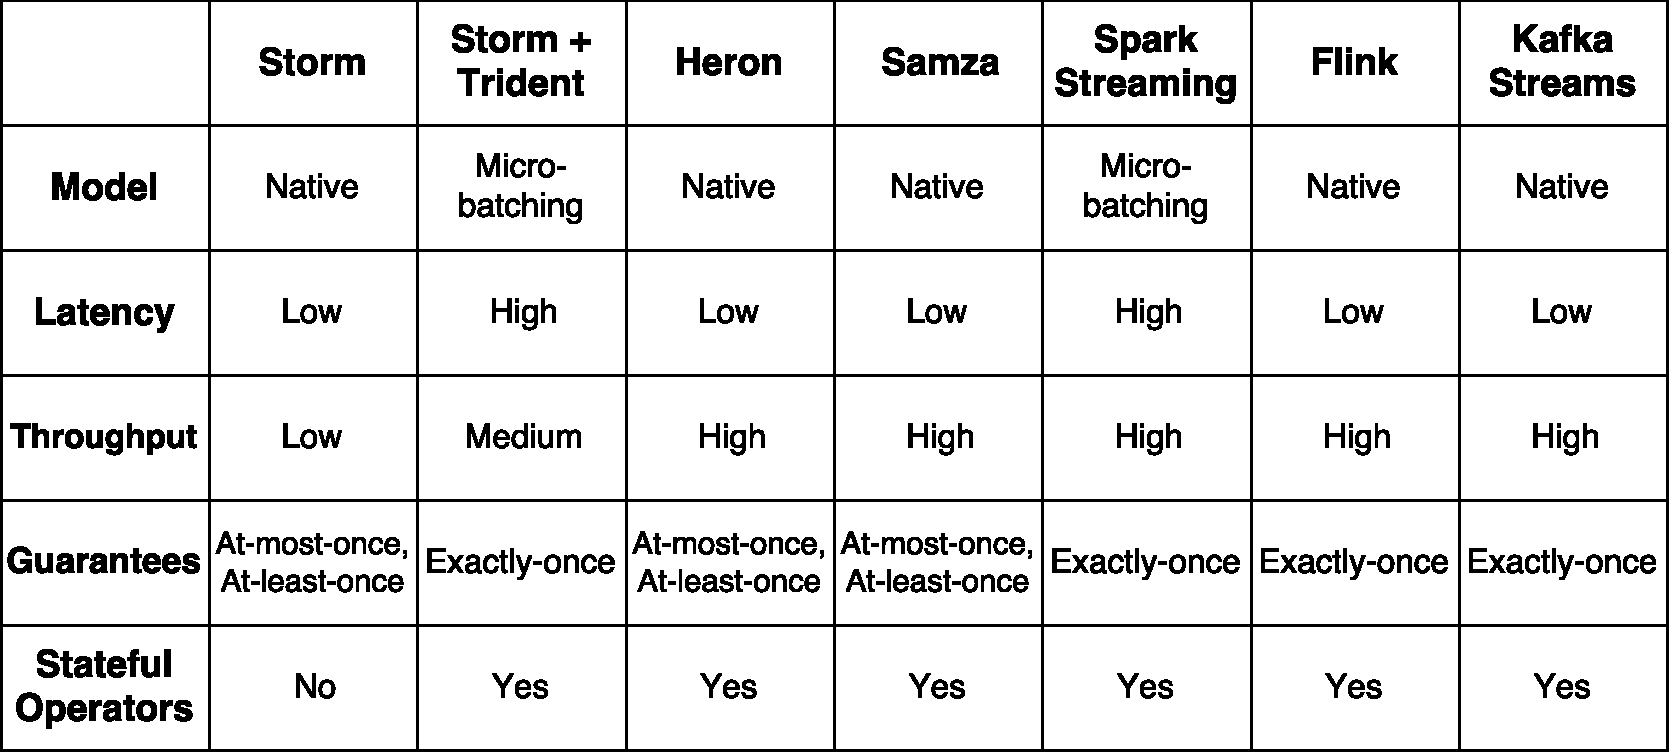
\includegraphics[width=1\textwidth]{images/streaming_engines.pdf}
 \caption{Streaming engines overview.}
\label{fig:streaming_engines_overview}
\end{figure}



An overview of the main features of the streaming frameworks discussed in the previous sections can be found in Figure \ref{fig:streaming_engines_overview}. We decided to evaluate Apache Spark Streaming, Flink and Kafka Streams. 
Apache Spark Streaming and Flink can be both good candidates because of their performances \cite{streamprocessingcomparison, yahoobenchmarkingonline, zalandobenchmarkingonline} and their maturity. They are also very flexible since they can be used as a single engine for both streaming and batch processing. Hence, they could be used as a single processing engine in the Lambda architecture. We chose also to test Kafka Streams because this system can be a good candidate for light-weight stream processing and we did not find any available benchmark of this system. 
%The result of the evaluation is available in Chapter 6. According to the results we obtained, Apache Flink is the streaming framework that better fits our uses cases. Thus, we decided to adopt Flink in our Cowbird architecture.

\section{Benchmarking Streaming Engines}
In this section we will portray the streaming engines benchmark framework we designed. We will report the results of the tests we performed on Apache Spark, Flink and Kafka Streams.
\subsection{The Benchmarking Framework}
\cite{yahoobenchmarkingonline, zalandobenchmarkingonline} designed a streaming engines benchmark that resembles their application scenario. Similar to what they have done, we designed a framework for evaluating streaming engines that recall our use cases. This approach can help us understanding which streaming framework is the most suitable for Cowbird. We tested Apache Spark Streaming (version 2.1.0), Apache Flink (version 1.2.0) and Kafka streams (Kafka version 0.10.2.0)

 \begin{figure}[h!]
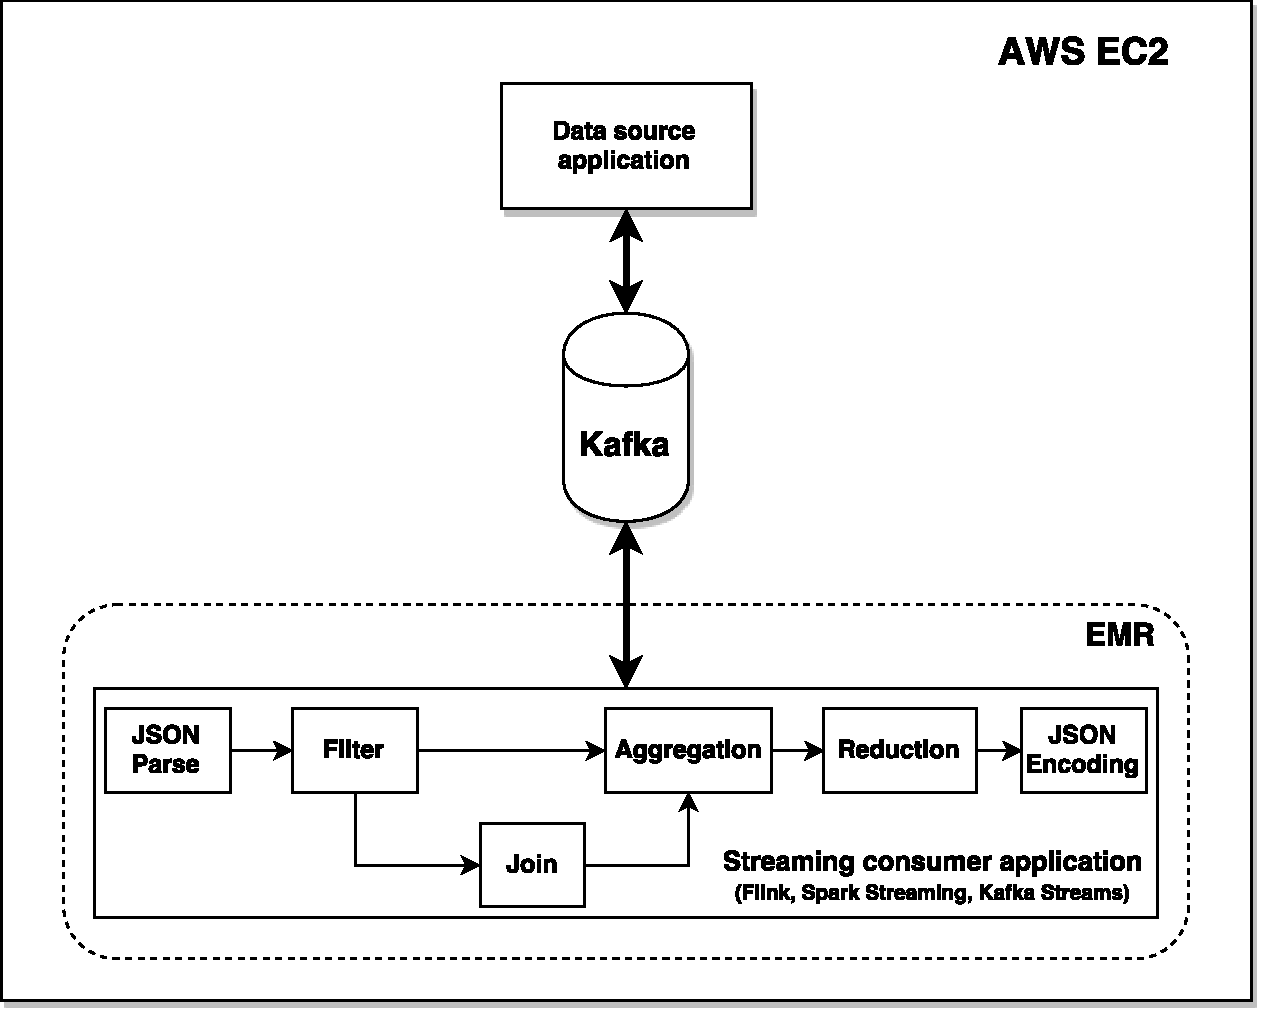
\includegraphics[width=1\textwidth]{images/benchmark.pdf}
 \caption{The streaming engines benchmark architecture.}
\label{fig:benchmark_architecture}
\end{figure}

Our benchmark framework contains (see Figure \ref{fig:benchmark_architecture}):
\begin{itemize}
\item A data source application that generates contents for a Kafka topic; each message generated contains an id that identifies a source, a double value, a reduction operation (i.e., MEAN, SUM, MAX and MIN), and the number of values required for applying the reduction operation (e.g., 1000 values coming from a source with a certain id). The data source application generates a certain number of events for a certain source and sends those to the Kafka broker. 
% batch??
The app can be tuned with some parameters provided by the user (e.g., number of sources, number of messages each source generates, the reduction operation to be performed on the data). 

%In Cowbird, instead, sensors data are generated This approach, indeed, can favorite the \emph{throughput}
%The SWAN framework processes sensors data values over a history time window while our benchmarking application process a certain number of values generated by a source. Hence, our benchmarking application can score a higher throughput since generated messages are sent in batch.

\item A streaming consumer application that runs on the streaming engine and applies the reduction operations. The application emits on Kafka the result for a certain source along with the time spent to compute the reduction operation. The time spent for computation is calculated as the difference between the time at the reduction evaluation and the timestamp of the first message received by Kafka from a certain source.
\end{itemize}

A consumer application has been designed for each of the three systems that have been tested. The consuming applications keep an \emph{incremental state} for each stream marked with a certain identifier. The incremental state stores only the partial result of the data that have been ingested so far into the system; this approach avoids to store all the records of data generated. The incremental state is calculated according to the reduction operator indicated for that stream. For example, in order to calculate the MEAN, the state will store the sum of the data values and the number of records that have flowed into the streaming engine. All the messages exhanged through the Kafka broker are in JSON format. The implementation of such benchmark framework can be found at \cite{streamingbenchmarkonline}

\subsection{Setup}
The evaluation has been done in a relatively simple setup on Amazon Web Services (AWS) \cite{amazonwebservicesonline}. The streaming engines are executed through EMR \cite{amazonemronline} on top of a small cluster composed of one master and two workers (m3.xlarge 4 vCPU, 15 GiB memory, 80 SSD GB storage each).
% The Kafka Streams application have been executed, instead, directly on three m3.xlarge instances using Amazon EC2 \cite{amazonec2online}.

Apache Kafka is executed in one broker instance along with Apache Zookeeper (m4.xlarge 4 vCPU, 16 GiB memory).

The streaming frameworks are executed using the default settings and we focused on writing correct, easy to understand programs without optimizing each streaming implementation to its full potential.

\subsection{Results}
We stressed all the three systems with different loads of messages containing double values. We use double values since many sensors produces measurements in such data format. In all the tests we performed the input messages have been processed using the MEAN history reduction mode. The batch duration in the Spark streaming was set to 1 second. In our tests, we focused on measuring how the tested systems react in terms of latency in situations of high input load.

\paragraph{}
Figure \ref{fig:results_100k} and Figure \ref{fig:results_1m} show the latency for various numbers of input messages per second. The results we obtained for Spark Streaming framework and Flink is similar to what was achieved by \cite{yahoobenchmarkingonline, zalandobenchmarkingonline}.

 \begin{figure}[h!]
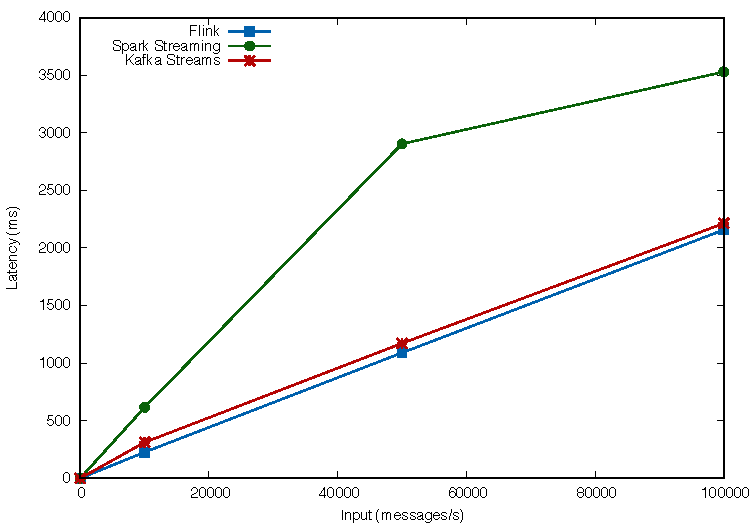
\includegraphics[width=1\textwidth]{images/engines_100k_cropped.pdf}
 \caption{Latencies evaluation up to 100K messages/s}
\label{fig:results_100k}
\end{figure}

 Kafka Streams performs very well and with a reasonable small input obtained performance similar to Apache Flink. Both Kafka Streams and Flink respond quite linearly. On the other hand, in Figure \ref{fig:results_100k} Spark Streaming behaves in a stepwise way; this could be a direct result from its micro-batching design. On drastically increasing the amount of input messages per second, all the three systems start suffering from the backpressure effect (the system is receiving data at a higher rate than it can process) also because of the limited setup configuration.
 
 \begin{figure}[h!]
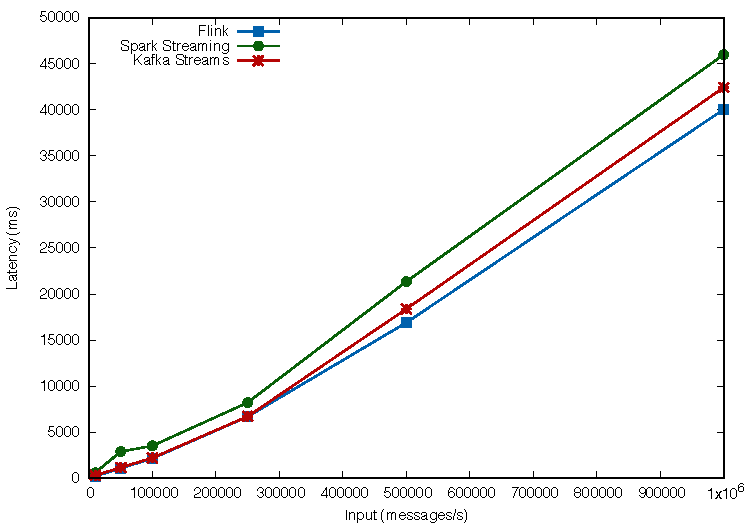
\includegraphics[width=1\textwidth]{images/engines_1m_cropped.pdf}
 \caption{Latencies evaluation up to 1M messages/s}
\label{fig:results_1m}
\end{figure}

 \begin{figure}[h!]
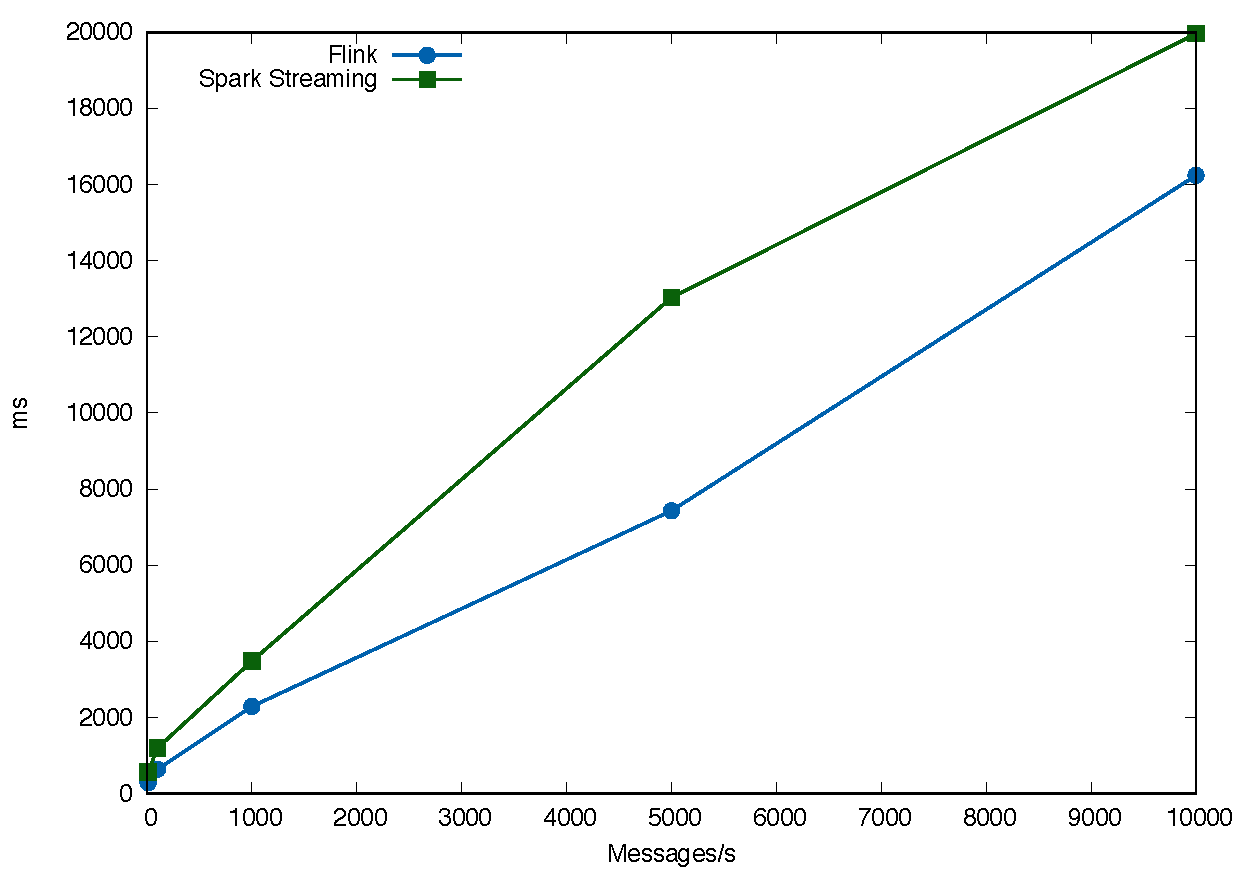
\includegraphics[width=1\textwidth]{images/join_cropped.pdf}
 \caption{Two streams JOIN-REDUCTION evaluation}
\label{fig:results_join}
\end{figure}


Figure \ref{fig:results_join} shows the evaluation result for join operations in Spark Streaming and Flink. In particular, the incoming streams of data (we set a window size of 1 second in Flink) are continuously joined with a set of 500MB pre-generated messages. The resulting streams of messages are then processed as usual. We notice that Flink has lower latency compared to Spark Streaming. We did not evaluate the join operation in Kafka Streams because such operator is not available for streams of data but only for tables.
\paragraph{}
The benchmark uses a naive setup and for this reason it can only give a sneak peek of the actual performance capabilities of the analyzed systems. Some of the achieved results are unacceptable or highly impractical for a real-time streaming application. However, this benchmark, even though executed on a relatively small scale, helped us understanding how the tested streaming engines can behave. Furthermore, in order to have a more detailed portrait of the tested engines fault tolerance and resources utilization should be evaluated as well. 
\paragraph{}
According to the results we obtained, Apache Flink is the streaming framework that better fits our uses cases. Nonetheless, it is important to outline that our naive benchmarking application is much less complex than the Cowbird framework. Furthermore, Cowbird evaluates sensors data records over a history time window while our benchmarking application processes a certain number of data values generated by a certain source without considering any windowing parameter.

%. Hence, our benchmarking application can score a higher throughput since generated messages are sent in batch.

%In Cowbird, instead, sensors data are generated This approach, indeed, can favorite the \emph{throughput}
%

\clearpage{\pagestyle{empty}\cleardoublepage}
\chapter{Design \& Implementation}
In the previous chapter we described some of the available stream processing frameworks. We evaluated some of them and eventually we decided to integrate Apache Flink in Cowbird. In this chapter we are going to illustrate how SWAN-Song expressions evaluation can be ported to Apache Flink. In general, we will portray how we extended Cowbird in order to accommodate data sensing and SWAN-Song expressions evaluation on a large scale. We will discuss the design choices we made and the technical challenges we tackled.  

\section{Hybrid-Cowbirds}
The existing Cowbird framework is designed to be executed on a single node machine. We designed a distributed architecture for supporting the real-time evaluation of a massive number of SWAN-Song expressions in Cowbird. We extended the Cowbird cloud architecture (see figure \ref{fig:distributed_cowbirds}) by adding two main components:
\begin{itemize}
\item \emph{Cowbird Fog}. A distributed layer responsible of receiving SWAN-Song evaluation requests from smartphones, polling sensors data and computing expressions. It is designed to bring expression evaluation as close as possible to the data generation in order to reduce latency. The Fog layer can decide to offload the SWAN-Song expression evaluation to the Streams layer according to some expression parameters (e.g. sensor data generation frequency, SWAN-Song expression time window). If an expression is offloaded to the Streams layer, the activated sensors threads in the Fog layer will \emph{asynchronously} publish their sensed data to a Kafka broker that mediates communications between the Fog and the Streams layer.
% GEOGRAPHICALLY STUFF
\item \emph{Cowbird Streams}. A high-performance and scalable layer for evaluating SWAN-Song expressions in real-time on a cluster using Apache Flink. It evaluates sensor data provided by the Fog layer and streamed through the Kafka broker. The result of the evaluation is sent back to Kafka and then made available to the Fog.
\end{itemize}

 \begin{figure}[h!]
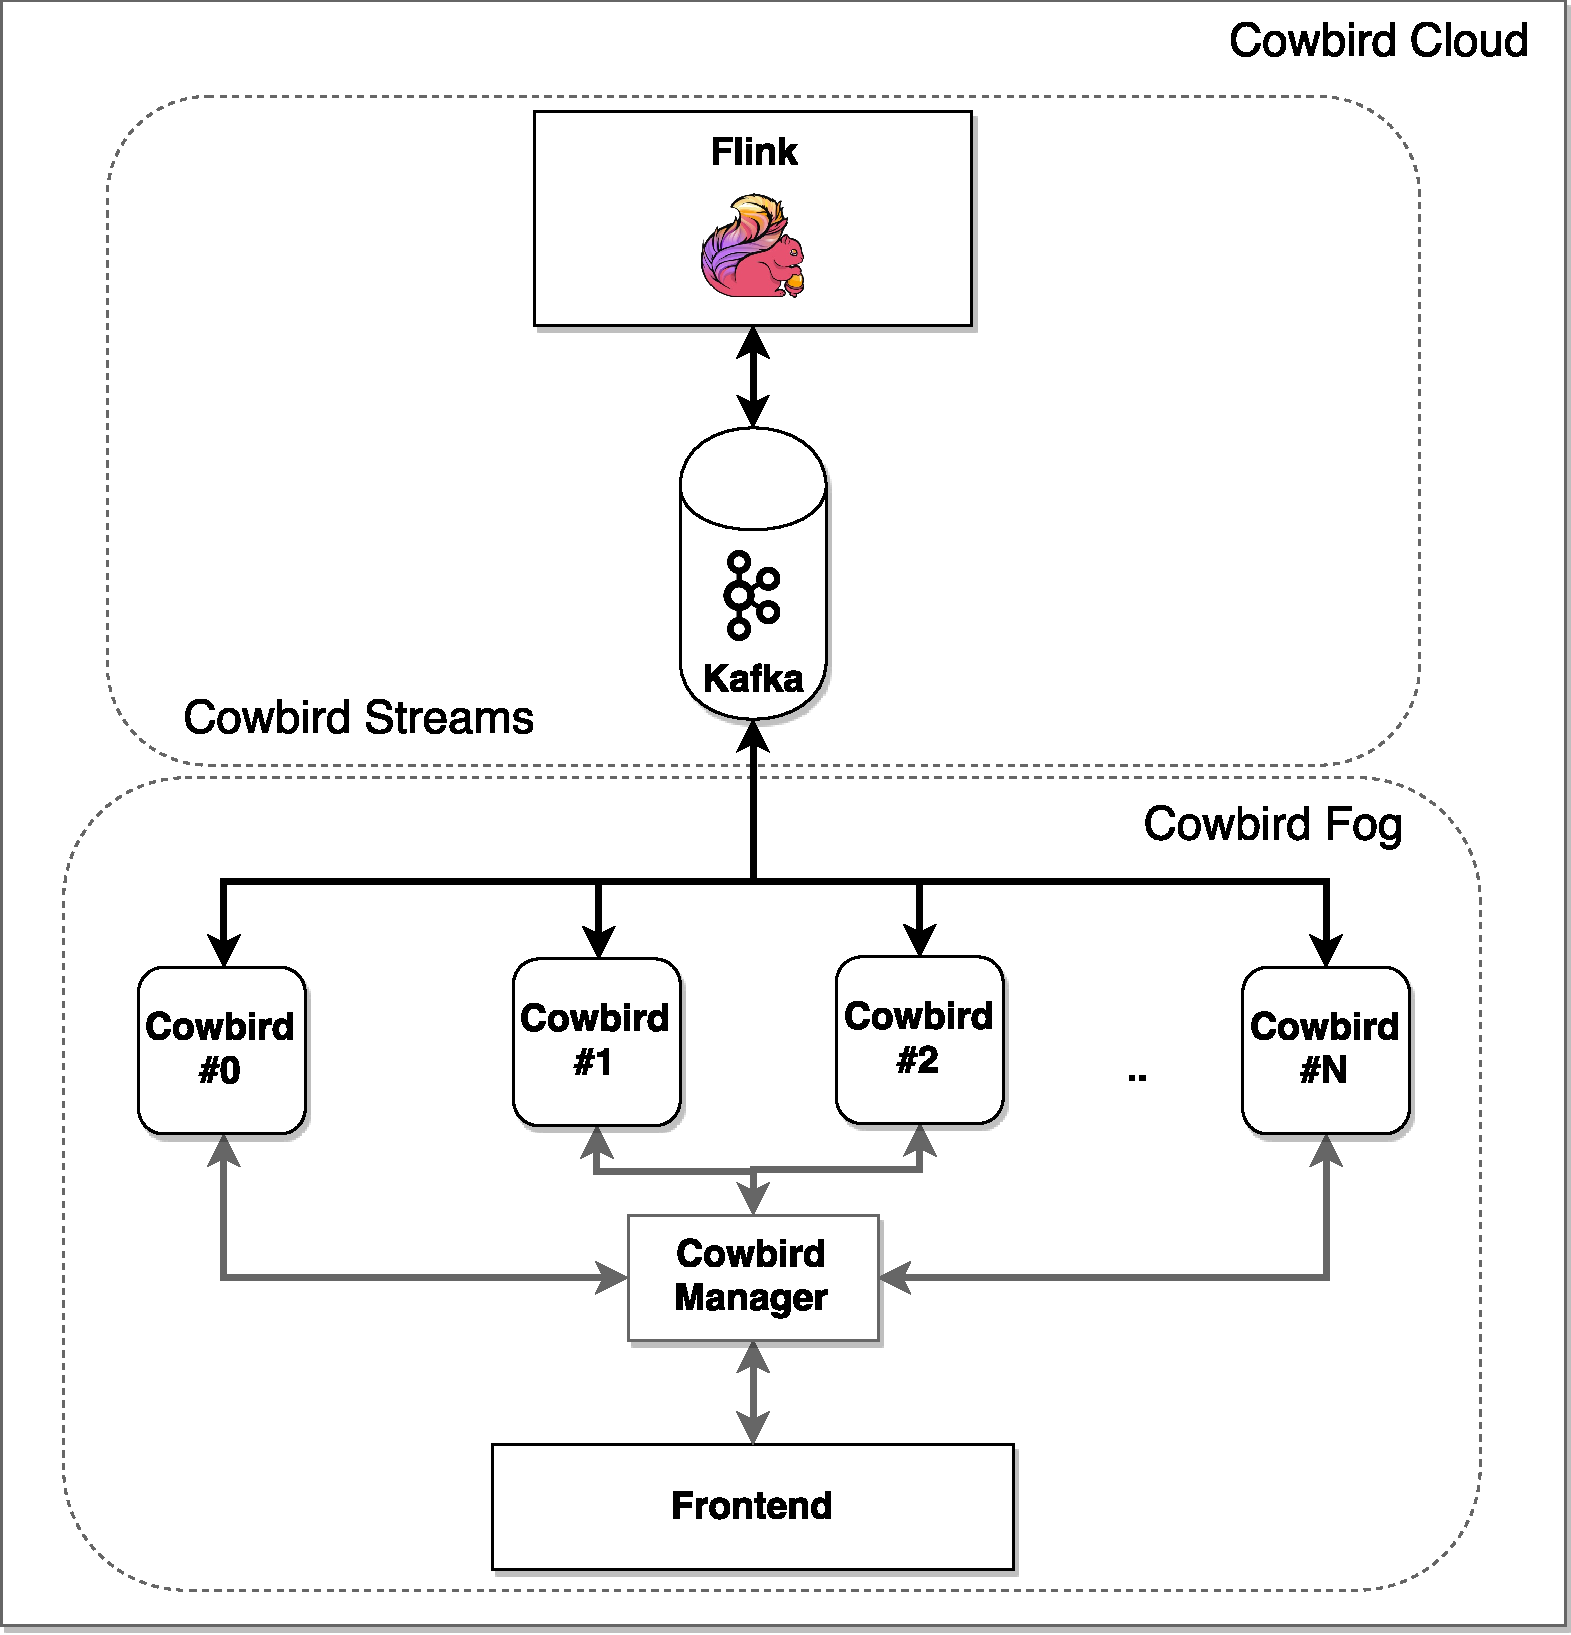
\includegraphics[width=1\textwidth]{images/cowbird_distributed.pdf}
 \caption{Hybrid-Cowbirds cloud architecture}
\label{fig:distributed_cowbirds}
\end{figure}

The Hybrid-Cowbirds model differs from the other streaming architectures described in Chapter 3 and Chapter 7. Hybrid-Cowbirds is a \emph{hybrid} architecture that combines large-scale modern streaming analysis techniques with more traditional processing systems. We added the Fog layer for performing some relative simple evaluation without involving an actual cluster system. The Fog layer can reduce latency bringing computation close to the data generation and to the users (and their smartphones). The Fog layer could be geographically distributed in order to provide high availability and high performance while the Streams layer will be a more centralized entity used for more complex evaluations that the Fog layer cannot handle. Furthermore, the Fog layer is extremely portable since it could be deployed on any device that runs a JVM. 

The remainder of this chapter will describe the internal details of the Hybrid-Cowbirds architecture. 

\section{Cowbird Fog}
In Chapter 2, we have seen that Cowbird makes large usage of threads for polling sensor data from external endpoints. This approach allows Cowbird to poll many different sources concurrently and in an asynchronous fashion. In Cowbird, a multi-threaded mechanism is adopted for the SWAN-Song expressions evaluation. However, having many active threads on a single computing node can incur in a certain system overhead. Furthermore, when polling live data, fetching data values might be delayed by multi-threading. It might be the case that new data records are available but Cowbird needs to wait for the relative sensor thread to become active again. A delay in fetching the data will induce a delay in processing the expression. In reaction to these issues, we decided to \emph{scale horizontally} the Cowbird cloud instance. 

 \begin{figure}[h!]
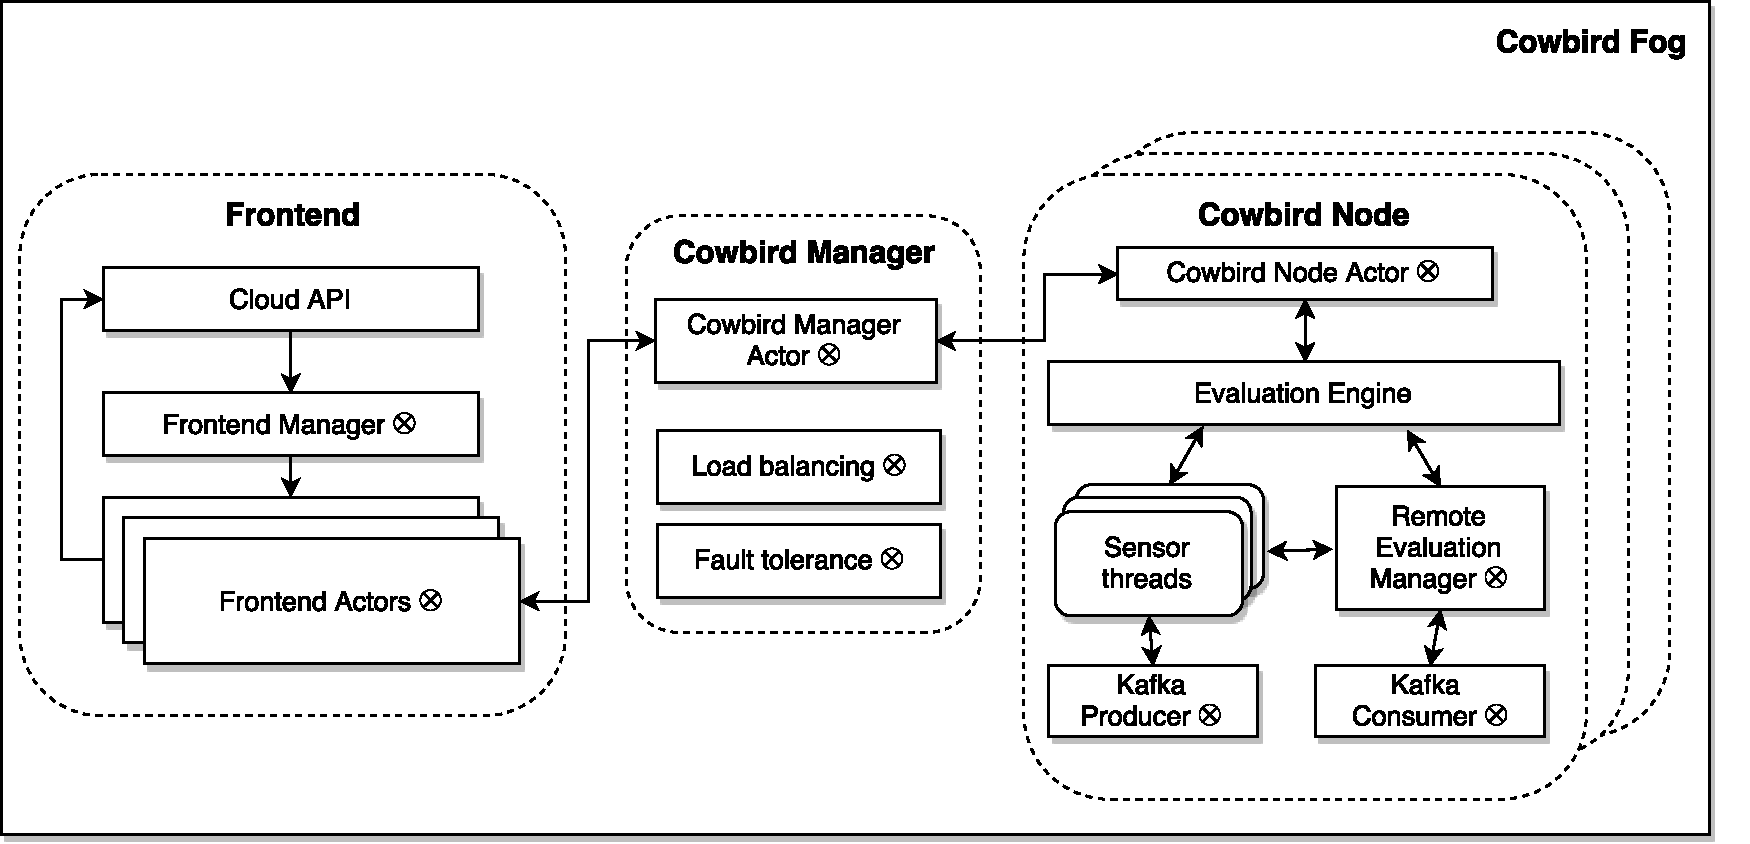
\includegraphics[width=1\textwidth]{images/fog_internals.pdf}
 \caption{Cowbird Fog internal details. New components and features are marked with $\otimes$.}
\label{fig:fog_internals}
\end{figure}

The Cowbird cloud instance is built using the Play framework with Java. For these reasons, we decided to scale out Cowbird using Akka \cite{akkaonline}. Akka is a set of open source libraries for building highly concurrent, distributed, and resilient message-driven applications using the \emph{actor model} \cite{actormodelbook}. The \emph{actor} is the primitive building block that forms the basis of the actor model. An actor is a concurrent entity that keeps an internal state that is not shared with other actors. The actor propagates data or events with other concurrent entities explicitly via asynchronous messages without blocking. Each actor processes the receiving messages one by one and it modifies its internal state. An actor is usually mapped to a thread; multiple actors can actually share the same system thread. The actor model can scale from processor cores to networks.
%Simplicity by design

In the original Cowbird implementation all its functionalities such as receiving SWAN-Song evaluation requests, sensing sensor data and computing the expressions are abstracted as a single instance. In the new distributed architecture, we structured the Cowbird Fog layer as follows (see Figure \ref{fig:fog_internals}):
\begin{itemize}
\item \emph{Frontend}. The Frontend is in charge of receiving the SWAN-Song expressions evaluation requests from smartphones. The Frontend mainly consists of a Play framework controller used in the original Cowbird implementation that routes a specific URL to a functionality. The Frontend is managed by the Frontend Manager. Every time a SWAN expression evaluation request is received at the Frontend, the Frontend Manager will spawn a \emph{Frontend Actor} responsible of the communication between the Frontend and the Cowbird Manager. In particular, the Frontend Actor registers the SWAN-Song to the Cowbird Manager and it will be notified when a new result value for the expression is available. The system also supports multiple active Frontend instances. %Scenario with multiple Frontend instances are possible and supported by the system.

\item	 \emph{Cowbird Node}. The Cowbird Manager assigns SWAN-Song expressions to be evaluated to a Cowbird Node. On receiving an expression, through the evaluation engine, the Cowbird Node will start the relevant sensor thread that will keep polling external web data from an endpoint. When the Cowbird Node computes new results for a registered expression, it will send back the results to the Cowbird Manager; the result is sent back to the manager with the same communication optimization strategy described in Chapter 2. We assume that the evaluation of the expression changes with low frequency and for this reason we direct all the result through the Manager. However, with a small change the result could be sent back directly to the Frontend. This optimization is possible since every component in the architecture is backed by an Akka actor. Messages between Akka actors can be exchanged directly even though they are running on different machines. The Cowbird node runs a \emph{Remote Evaluation Manager} that determines whether or not a SWAN-Song expression should be offloaded for evaluation to the Cowbird Streams layer. A SWAN-Song expression (or just a part of it) is offloaded to the Streams layer if it refers to a sensor marked as \emph{high-frequency} or if the expression has to be evaluated over a time window that is longer than a certain configurable threshold (e.g. 10 minutes).

The Cowbird Node integrates a Kafka \emph{producer} and a Kafka \emph{consumer} that coordinate the communication with the Streams layer. 

Cowbird Nodes can be dynamically added or removed for horizontal scalability.

\item \emph{Cowbird Manager}. The Cowbird Manager is responsible for the coordination of the workload distribution among all the Cowbird nodes in the system. When a new SWAN-Song expression evaluation request is received from the Frontend, the manager assigns it to the \emph{least-busy} Cowbird node in the network (i.e., the Cowbird Node with the minimum number of active threads). The Cowbird Manager is also responsible for monitoring the entire Fog layer. The manager detects failing Cowbird Nodes and Frontend(s). In reaction to these scenarios, the manager can redistribute the workload to another active node in the system or it can stop the sensor data sensing and expression evaluation in case of a failing Frontend. The Cowbird Manager can be deployed in \emph{high-availability mode} to guarantee a certain level of fault-tolerance. In this scenario, when the manager fails one of the Cowbird Node will be elected as the manager. 
\end{itemize}

The above described components can be deployed all three in a single machine or they can be distributed over many computing nodes for achieving better performance. Many deployment optons are possible and thus the Fog layer is extemely versatile. This is possibile thanks to the Akka framework flexibility. The scenario where different Fogs are distributed geographically for performance and availability is also possible. Hence, Cowbird cloud could meet the concept of \emph{fog computing} \cite{fogcomputingBonomi2012}. 
%GEOGRAPHY

\section{Cowbird Streams}
The Cowbird Streams layer is the high-performance module of our new Cowbird implementation. As we already mentioned, it consists of a Kafka cluster and an Apache Flink application. The Kafka cluster is responsible for receiving the sensed data from the Fog layer; the Flink application processes the incoming streams and writes the result of the evaluations back to Kafka.

The Cowbird Streams layer needs the Fog layer in order to exploit its sensing capabilities. 

We ported the SWAN-Song evaluation mechanism to Apache Flink. In particular, we implemented the core SWAN-Song functionalities using the Flink API. In order to bring SWAN-Song evaluations on top of Flink, we need to stream the registered expressions along with the sensed data from the Fog layer through Kafka. The Fog layer exchanges \emph{messages} with the Flink job running the SWAN logic. All the messages are exchanged in JSON format through the Kafka broker. We designed three different type of messages:
\begin{itemize}
\item \emph{Sensor message}. Every time a sensor thread that belongs to a SWAN-Song assigned for evaluation to the Streams layer generates a data record it is encapsulated in a sensor message. The sensor message contains the data value and the identifier of the expression it belongs to. Each SWAN-Song expression has an unique identifier assigned by the Cowbird Manager.
\item \emph{Control message}. The control message is sent from the Cowbird Node when it wants to register/deregister a SWAN-Song expression to the Streams layer. It contains the identifier of the expression and the type of history reduction along with the window size.
\item	 \emph{Result message}. The result message contains the result of the evaluation. It is sent from the Flink job every time a new result is available for a certain expression.  
\end{itemize}

When the Cowbird Node receives a new expression to evaluate from the Cowbird Manager, the remote evaluation engine decides if the expression or part of it should be evaluated by the Streams layer. If this is the case, the Cowbird Node will register the SWAN-Song through a control message to the Streams layer. The evaluation engine will then start the relative sensors threads; the sensed data instead of being stored and evaluated locally will be sent asynchronously to the Flink job running on Cowbird Streams. The Cowbird Node will be notified when a new result for the registered expression is available.
\subsection{SWAN-Song Evaluation on Cowbird Streams}
Implementing the entire SWAN logic on top of a streaming engine can be very inefficient. SWAN expressions are parsed by the Cowbird Fog and parsing them again would introduce extra overheads. 
% the expression on the Streams layer  Implementing from scratch the entire SWAN stack functionalities (e.g. parsing expression, expression evaluation) on Apache Flink would require a lot of effort and it would be probably useless. 
Thus, we designed the system in a way that the Fog layer can offload only some \emph{well-known} types of SWAN expressions (or subexpressions of a more complex expression) to the Streams. The Fog layer will then be in charge to compute the final result of an expression with the partial results computed by the Streams layer. In particular, our Streams layer is capable of computing the following types of SWAN-(sub)expressions: SWAN simple value expression, SWAN simple tristate comparison expression and SWAN complex tristate comparison expression. 

\subsubsection{SWAN Simple Value Expression} 
This is the simplest kind of SWAN-Song expression that can be evaluated by the Cowbird Streams layer. Such expressions only contain the basic SWAN predicates but they don't support the ALL or ANY reduction mode. An example of such expressions can be:
\begin{equation}\label{eq:simpleexpression}
cloud@thingspeak:field?channelid='1'\#field='1'\big\{MEAN,3600000\big\}
\end{equation}

If a SWAN simple value expression is part of a more complex expression, the final result would be computed by the Fog layer when the result of the simpler expression is evaluated on the Streams and then sent back. For example, consider the following expression:
\begin{equation}\label{eq:simpleexpression_comparison}
cloud@thingspeak:field?channelid='1'\#field='1'\big\{MEAN,3600000\big\} > 50.0
\end{equation}

In SWAN-Song (\ref{eq:simpleexpression_comparison}) only the left-side of the expression would be offloaded to the Streams layer. The final comparison (if the MEAN value is greater than 50) would be computed on the Fog layer when the result of the left-side expression is received back.

\subsubsection{SWAN Simple TriState Comparison expression} 
The SWAN simple tristate comparison expression is a comparison expression that consists of a SWAN-Song expression with ANY or ALL history reduction mode and a constant value. For example, consider the following expression:
\begin{equation}\label{eq:simple_comparison_expression_comparison}
cloud@thingspeak:field?channelid='1'\#field='1'\big\{ANY,3600000\big\} > 50.0
\end{equation}

The expression (\ref{eq:simple_comparison_expression_comparison}) is completely evaluated on the Streams layer and when a result is available it is pushed back to the Cowbird Fog layer. This approach is essential in order to prevent the Cowbird Streams layer to return a long list of time-stamped values. 

In order to maximize efficiency and performance some shortcuts have been implemented in the evaluation of such expression. In particular, in case of a simple comparison expression that has the ANY history reduction mode the expression is evaluated immediately when a data record that makes the expression TRUE flows into the Streams layer (without evaluating also the other data values generated within the window history length). On the other hand, a simple comparison expression that has the ALL history reduction mode is immediately evaluated if a record that makes the expression FALSE enters the system.


\subsubsection{SWAN Complex TriState Comparison Expression} 
The SWAN complex tristate comparison expression represents a more complex type of comparison expression. It consists in comparison expressions that involve the ANY or ALL history reduction modes. For example, consider the following expressions:
\begin{equation}\label{eq:complex_comparison_expression_comparison}
cloud@mysoundsensor1\big\{ANY, 3600000\big\} > cloud@mysoundsensor2\big\{ALL, 2400000\big\} 
\end{equation}
The expression (\ref{eq:complex_comparison_expression_comparison}) is completely evaluated on the Cowbird Streams layer (if off-loaded).

\subsection{SWAN-Song Streaming-Oriented Evaluation}
The new Cowbird implementation supports the same set of operations provided by the previous generation of Cowbird cloud. In fact, offloading the three types of (sub)expressions described above to the Streams layer and letting the Fog layer compute and aggregate the partial results (if applicable) leads to the same exact result of the traditional SWAN evaluation.

The SWAN features are implemented on Apache Flink using its low-level operations API (i.e. ProcessFunction). The Flink implementation keeps an internal state for each stream of sensors data using the RocksDB key-value store \cite{rocksdbonline}. This state backend can store very large state that exceeds memory and it spills to disk efficiently. All the SWAN features are implemented in Apache Flink using \emph{processing time} in order to guarantee real-time performance even if the data records are delayed. However, event time can be configured by the user.

We designed two different implementations of how the Cowbird Streams processes SWAN-Song simple value expressions. One implementation, that we called \emph{core implementation}, reproduces exactly the way SWAN-Song expressions are processed in the original SWAN framework. In particular, for each expression the system collects all the sensor values generated within the history time window and the history reduction mode is then applied. This approach is very precise and it allows the system to continuously generate an expression result based on the values stored that belong to the history time window. However, this approach is not really \emph{streaming-oriented}; in fact, streaming applications should incrementally aggregate partial results while new data records enter the system. In reaction to this, we designed a \emph{streaming-oriented} SWAN-Song evaluation that can be executed on Cowbird Streams. The philosophy of this implementation is to store the partial results of each stream of data related to a SWAN-Song expression instead of all the data values generated by the sensor within a certain history time window. For example, if we want to compute the MEAN value of the data generated by a sound sensor in the last five seconds we just need to count how many data occurrences have been generated by the sensor and the sum of the data values. Another example can be an expression with the MAX history reduction mode set. In this scenario, we just need to store a partial maximum value and every time a greater value enters the system we can simply replace the partial maximum. This approach can prevent the system to leave the ground to the back pressure effect and it drastically reduces the amount of storage required by each stream for keeping its internal state. 
% This approach can drastically reduce the space complexity of our streaming application; complexity that could explode when we deal with very large streams of data. 

The MAX, MIN, MEAN history reduction modes can very easily adopt this streaming-oriented evaluation approach. However, the MEDIAN operator requires all the data records in order to compute the median value. We decided to design a MEDIAN operator implementation that approximates the median of the data streams. In some contexts, such as biology or genetics, robust statistical procedures are required to process data. Applications that use these kinds of sensitive data are not really suitable for adopting a MEDIAN approximatated value. However, in scenarios such as enviromental monitoring, agriculture and industrial monitoring applications \cite{approximationtimeseries} an approximation could be a very attractive alternative. In fact, these types of applications are usually characterized by a large number of sensing devices and they can tolerate a lower level of accuracy. In the literature, there are many approaches designed to approximate sensor values \cite{approximateprobabilistic, approximationdatabase}. 
%These techniques are very attractive for some domains where a large number of sensing devices are involved such as enviromental monitoring, agriculture and industrial monitoring applications \cite{approximationtimeseries}. 
We approximated the MEDIAN history reduction mode using the remedian algorithm \cite{remedian}. This algorithm has been proven to be very efficient \cite{remedianfurtheranalysis} and it only requires $\mathcal{O}(\log{}n)$ space to compute the median value. This technique can be used for both batch and stream processing. 

The remedian algorithm requires \emph{k} arrays of size \emph{b} that are continuously reused. The data enter at the first array that is filled with the first \emph{b} observations. Then, the median of these \emph{b} observations is stored in the first element of the second array. The first array is then used again for the second group of \emph{b} observations, the median of which will be put in the second position of array 2. After some time array 2 is full too, and its median is stored in the first position of array 3, and so on. When the \emph{k}-th array is complete its median becomes the final estimate. If the input data cannot fill the entire matrix, the estimation of the median is calculated as a \emph{weighted median} of the stored data. In particular, the $n_1$ numbers in the first array have weight 1, the $n_2$ numbers in the second array have weight b, and the \emph{$n_k$} numbers in the last array have weight $b^{k-1}$.

In our SWAN-Song streaming oriented evaluation implementation, the \emph{k} and \emph{b} value of the remedian matrix can be configured by the user. However, we set as default values \emph{k}=15 and \emph{b}=11 as described in \cite{remedian}. With these values our system is able to process the (re)median value of a stream of data that has up to $11^{15}$ observations with just a $11 \times 15$ matrix. 

The SWAN-Song streaming-oriented evaluation is much more efficient than the traditional implementation and it is more suitable for real-time streaming applications. However, the new implementation introduces a lower degree of accuracy for the MEDIAN operator. Furthermore, the SWAN-Song streaming evaluation operates only over \emph{fixed} or \emph{aligned} time windows (i.e., the reduction is applied only across all the data ingested during the window of time in question). Since the reduction is calculated continuously aggregating incoming data within a time frame, an expression result is emitted at the end of each time window (e.g., with a 5 seconds window size, a result is emitted every 5 seconds).

The SWAN-Song streaming-oriented evaluation is particularly suitable for applications that can tolerate a certain lack of accuracy and that operate at regular time intervals. Mission critical applications, where a better level of accuracy is required, could instead use the traditional implementation. Both the implementations are available in the Cowbirds Streams layer and they could be deployed together allowing different type of sensors to use the most convenient evaluation strategy.

\section{Summary}
In this chapter we described how we extended the existing Cowbird cloud instance for supporting a massive volume of SWAN-Song expression evaluations. We called the new Cowbird cloud architecture \emph{hybrid} since it adds an extra computational layer to the traditional streaming architecture.

The Cowbird Fog module brings the evaluations closer to the sensor data generation. The Fog layer is also extremely scalable since Cowbird nodes can be dynamically added and removed at run time. Furthermore, Fog(s) could be put closer to the user to improve availability and performance. 

The Cowbird Streams is the high-performance component of the architecture. The Streams layer is powered by Apache Flink that we demonstrated to be the streaming framework that best meets our scenario. The Cowbird Streams supports two different SWAN-Song evaluation strategies: a \emph{core implementation} that exactly reproduces the SWAN framework and a more \emph{streaming-oriented} implementation. Both implementations can be adopted according to the type of sensor which the data is being evaluated. The Cowbird Streams is designed to accommodate \emph{long-running} SWAN-Song expressions or expressions characterized by very \emph{high-frequency} sensors. 

The Hybrid-Cowbirds implementation is available at \cite{distributedcowbirdsonline}.



\clearpage{\pagestyle{empty}\cleardoublepage}
%\include{Architettura}
%\clearpage{\pagestyle{empty}\cleardoublepage}
%\include{TED}
%\clearpage{\pagestyle{empty}\cleardoublepage}
%!TEX encoding = UTF-8 Unicode\pagestyle{empty}
%\clearpage{\pagestyle{empty}\cleardoublepage}
%\include{APIs}
%\clearpage{\pagestyle{empty}\cleardoublepage}
%\include{Test}
%\clearpage{\pagestyle{empty}\cleardoublepage}


%%%%%%%%%%%%%%%%%%%%%%%%%%%%%%%%%%%%%%%%%non numera l'ultima pagina sinistra
\clearpage{\pagestyle{empty}\cleardoublepage}
%%%%%%%%%%%%%%%%%%%%%%%%%%%%%%%%%%%%%%%%%per fare le conclusioni
\chapter*{Conclusions and future work}
%%%%%%%%%%%%%%%%%%%%%%%%%%%%%%%%%%%%%%%%%imposta l'intestazione di pagina
%\rhead[\fancyplain{}{\bfseries
%CONCLUSIONI}]{\fancyplain{}{\bfseries\thepage}}
%\lhead[\fancyplain{}{\bfseries\thepage}]{\fancyplain{}{\bfseries
%CONCLUSIONI}}
%%%%%%%%%%%%%%%%%%%%%%%%%%%%%%%%%%%%%%%%%aggiunge la voce Conclusioni
                                        %   nell'indice
%\addcontentsline{toc}{chapter}{Conclusioni e sviluppi futuri} 
%\input{ConclusionAndFutureWorks}


 %\cite{K3,K4}.
%%%%%%%%%%%%%%%%%%%%%%%%%%%%%%%%%%%%%%%%%imposta l'intestazione di pagina
%\renewcommand{\chaptermark}[1]{\markright{\thechapter \ #1}{}}
%\lhead[\fancyplain{}{\bfseries\thepage}]{\fancyplain{}{\bfseries\rightmark}}
%\appendix                               %imposta le appendici
%\chapter{Configurazioni utilizzate nei test}               %crea l'appendice


%%%%%%%%%%%%%%%%%%%%%%%%%%%%%%%%%%%%%%%%%non numera l'ultima pagina sinistra
\printbibliography 
\clearpage{\pagestyle{empty}\cleardoublepage}
\chapter*{Acknowledgement}
Grazie.
\end{document}
